\subsubsection{Brute-Force-Tarpit}
Neben der Harvester-Tarpit war auch die Brute-Force-Tarpit erfolgreich. Insgesamt wurden 7.051 Loginversuche getätigt. Hierbei wurden aus zehn verschiedene Benutzernamen und 1.107 verschiedenen Passwörtern 3.793 verschiedene Kombinationen gewählt, somit wurde jede Kombination im Schnitt mehrfach probiert. In den Tabellen \ref{tab:top-ben} und \ref{tab:top-pass} sind die häufigsten Benutzernamen und Passwörter aufgezeigt, welche in der simulierten Wordpressloginform eingegeben wurden.
\begin{table}[htb!]
	\centering
	\begin{tabular}{c|c}
		\textbf{Benutzername}&\textbf{Anzahl an Versuchen}\\\hline
		admin & 2340\\
		maturaprojekt & 1308\\
		test & 1246 \\
		webmaster & 1052\\
		root & 1052 \\
		administrator & 46 \\
	\end{tabular}
	\caption{Die am häufigsten eingegebenen Benutzernamen}
	\label{tab:top-ben}
\end{table}
\begin{table}[htb!]
	\centering
	\begin{tabular}{c|c}
		\textbf{Passwort}&\textbf{Anzahl an Versuchen}\\\hline
		admin & 24\\
		PASSWORD & 24\\
		nicole & 19\\
		michael & 19\\
		daniel & 18\\
		jessica & 17\\
		111111 & 15\\
		lovely & 15\\
		ashley & 15\\
		iloveyou & 14\\
		... & ...\\
		THOMAS & 8\\
	\end{tabular}
	\caption{Die am häufigsten eingegebenen Passwörter}
	\label{tab:top-pass}
\end{table}
\\Analog hierzu sind in Tabelle \ref{tab:top-pass-splash} die zehn häufigsten Passwörter von 2017 aufgezeigt.\footnote{Die zehn häufigsten Passwörter laut SplashData, \href{https://13639-presscdn-0-80-pagely.netdna-ssl.com/wp-content/uploads/2017/12/Top-100-Worst-Passwords-of-2017a.pdf}{hier geht es zur kompletten Liste:} (\url{https://13639-presscdn-0-80-pagely.netdna-ssl.com/wp-content/uploads/2017/12/Top-100-Worst-Passwords-of-2017a.pdf}).}
\begin{table}[htb!]
	\centering
	\begin{tabular}{c|c}
		\textbf{Platz}&\textbf{Passwort}\\\hline
		1 & 123456\\
		2 & Password\\
		3 & 12345678\\
		4 & qwerty\\
		5 & 12345\\
		6 & 123456789\\
		7 & letmein\\
		8 & 1234567\\
		9 & football\\
		10 & iloveyou\\
	\end{tabular}
	\caption{Die am häufigsten genutzten Passwörter laut SplashData}
	\label{tab:top-pass-splash}
\end{table}
Vergleicht man nun Tabelle \ref{tab:top-pass} mit Tabelle \ref{tab:top-pass-splash}, so kann man deutlich erkennen, dass unter anderem die Standardpasswörter aus Tabelle \ref{tab:top-pass-splash} häufig probiert wurden. Dies lässt sich vor allem dadurch erklären, dass die Betreiber solcher Webcrawler bewusst ihre Liste der zu probierenden Passwörtern mit solchen \glqq typischen Passwörter\grqq\space füllen. Die vielen Vornamen, welche in das Passwortfeld eingetragen wurden, lassen sich jedoch nicht erklären. Wahrscheinlich hat ein Webcrawler eine sogenannte Wörterbuchattacke ausgeführt, sprich er hat Passwörter probiert, welche man in einem Wörterbuch auffinden kann. Hierzu zählen selbstverständlich auch Vornamen. Beeindruckend ist jedoch die Tatsache, dass Webcrawler auch meinen Vornamen als Passwort ausprobiert haben. Meinen Vornamen herauszufinden ist für einen Webcrawler ein leichtes Spiel: Der Meta-Tag \emph{author} in der HTML-Seite enthält den Wert \emph{Thomas Brixen}. Das beeindruckende und zugleich unerklärliche ist jedoch, dass kein einziges mal, weder als Benutzernamen, noch als Passwort, das Wort \emph{Brixen} probiert wurde, obwohl es, wie auch mein Vorname, der Wert des Metatags \emph{author} ist. Selbstverständlich könnte ein Webcrawler den Inhalt des Metatags durch einen Filter laufen lassen und merken, dass \emph{Brixen}, im Gegensatz zu \emph{Thomas}, kein Name ist. Des Weiteren könnte ein Webcrawler auch anhand der IP-Adresse den ungefähren Standort des Webservers zurückverfolgen und würde dann merken, dass \emph{Brixen} eine Stadt im unmittelbaren Umfeld ist. Beides rechtfertigt jedoch nicht, das Wort \emph{Brixen} als einen potentiellen Benutzernamen oder Passwort auszuschließen und deshalb nicht zu probieren.
\begin{table}[htb!]
	\centering
	\begin{tabular}{c|c}
		\textbf{User-Agent (nur Browser)}&\textbf{Anzahl an Loginversuchen}\\\hline
		Firefox/40.1 & 3.755 \\
		Firefox/3.0.15 & 3.152 \\
		\emph{Weitere User-Agents}\footnote{Die restlichen Loginversuche stammen wurden mit verschiedenen User-Agents ausgeführt und sind in ihrer Anzahl so klein, dass sie für die Auswertung nicht relevant sind.} & 144
	\end{tabular}
	\caption{Die User-Agents (nur Browser) mit welchen Loginversuche getätigt wurden}
	\label{tab:top-user-agent}
\end{table}
\\Aus Tabelle \ref{tab:top-user-agent} lässt sich des Weiteren eindeutig erkennen, dass für die Angriffe hauptsächlich zwei Versionen des Browsers Firefox, nämlich die Versionen 40.1 und 3.0.15, verantwortlich waren. Jedoch veröffentlichte Mozilla beispielsweise nie eine Version 40.1 von Firefox\cite{firefox-versions}. Nach kurzer Recherche zeigt sich, dass der User-Agent Firefox/40.1 dafür bekannt ist, weltweit Loginversuche auf Webseiten, welche Wordpress verwenden, zu tätigen\cite{firefox-40-1}. Viele vermuten hinter Firefox/40.1 ein Botnetz\footnote{Ein Botnetz ist eine Ansammlung von Endgeräten, Router, PCs, Smartphones, etc., welche von einem Angreifer aus der Ferne kontrolliert werden können. Durch eine Schadsoftware, welche beispielsweise zuvor über E-Mails verbreitet wurde, werden nach und nach immer mehr Endgeräte in dieses Botnetz aufgenommen. Ein großes Botnetz kann schnell mehrere Tausend Endgeräte umfassen. Meist werden Botnetze für einen DDoS-Angriff verwendet, bei welchem zu einem Zeitpunkt X die infizierten Endgeräte simultan eine Ressource auf einem Webserver anfragen, mit dem Ziel, dass dieser Webserserv die Anfragen nicht stemmen kann und zusammenbricht.}, zu welchem Endgeräte auf der ganzen Welt zusammengeschlossen wurden\cite{wordpress-botnetz}. Diese Vermutung bestätigte sich im Verlaufe dieses Versuches. In der Zeit vom 25. bis zum 28. Februar 2018 wurde VEVETA Opfer eines Angriffes eines Botnetzes. Endgeräte aus 152 verschiedenen Ländern versuchten sich über die Wordpressloginform anzumelden und tappten dabei in die Falle: Die Brute-Force-Tarpit fing sie und loggte ihre Loginversuche mit. Hierbei schienen fast ausschließlich User-Agent mit dem Browser Firefox/40.1 auf.\newpage
Die Angriffe des Botnetzes kamen hierbei, wie bereits erwähnt, aus 152 verschiedenen Ländern, was in 
%Tabelle \ref{tab:top-countries-botnetz} und 
Abbildung \ref{fig:botnetz-karte} nochmals verdeutlicht wird:\\
%\begin{table}
%	\centering
%	\begin{tabular}{c|c}
%		\textbf{Land}&\textbf{Anzahl der Loginversuch}\\\hline
%		Brasilien & 266\\
%		Indien & 252\\
%		USA & 202\\
%		Philippinen & 167\\
%		Italien & 114\\
%		Malaysia & 102\\
%		Frankreich & 100\\
%		Algerien & 94\\
%		Spanien & 80\\
%		Serbien & 78
%	\end{tabular}
%	\caption{Die Länder, welche während des Angriffes des Botnetzes die meisten Loginversuche tätigten}
%	\label{tab:top-countries-botnetz}
%\end{table}
\begin{figure}[H]
	\centering
	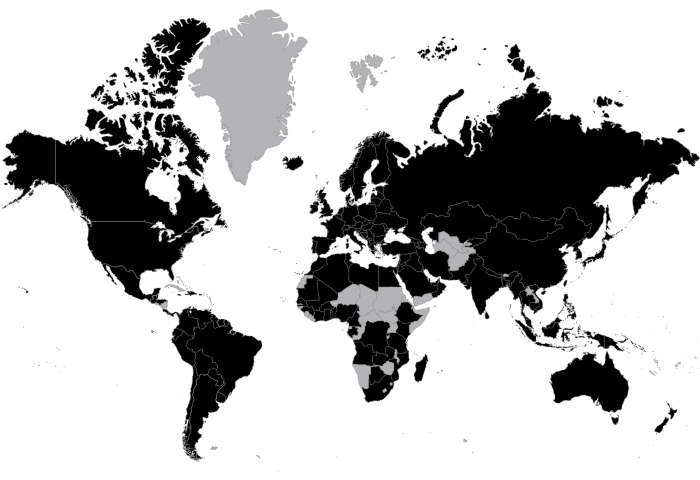
\includegraphics[width=8.45cm]{img/botnetz-angriffe-karte-1920-1080.png}
	\caption{Länder aus denen der Angriff des Botnetzes stammte (schwarz markiert)}
	\label{fig:botnetz-karte}
\end{figure}
Hierbei kann man in Abbildung \ref{fig:botnetz-karte} deutlich erkennen, dass nahezu jedes Land Bestandteil dieses Botnetzes ist. Sowohl  Internetnutzer in Schwellenländern als auch in Industriestaaten wurden Opfer einer schadhaften Software, welche dann später diesen Angriff koordiniert hat.
%TODO:
%\newpage
%EVTL FA DEN ZEUG DO SCHREIBEN
%\begin{table}
%	\centering
%	\begin{tabular}{c|cc}
%		\textbf{Anzahl der Anfragen}&\textbf{Datei}&\textbf{Methode}\\\hline
%		4.574 & / & GET\\
%		3.993 & /wp-login.php & GET\\
%		3.919 & /wp-login.php & POST\\
%		3.782 & /xmlrpc.php & POST\\
%		3.152 & //wp-login.php & POST\\
%		1.862 & - & ---\\
%		1.737 & /wp-admin/ & GET\\
%		1.722 & /test/wp-admin/ & GET\\
%		1.715 & /wordpress/wp-admin/ & GET\\
%		1.712 & /blog/wp-admin/ & GET
%	\end{tabular}
%	\caption{Die am häufigsten angefragten Dateien}
%	\label{tab:top-hits-wordpress}
%\end{table}